\chapter{Test}\label{Test}

\testing{EMG Thresholds R\ref{test:EMG}}\label{test:Connectiontest}
\begin{figure}[H]
    \centering
    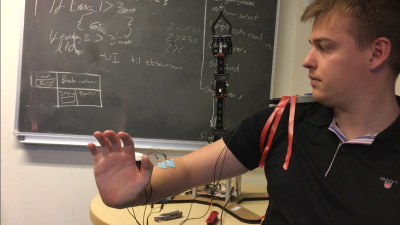
\includegraphics[width=10cm,height=5cm]{Figures/Technical_figures/image2.png}
    \caption{The user sits in a contracted position for 3 minutes}
    \label{fig:connectiontest}
\end{figure}
\subsection*{Layout}
To set with three electrodes in each set, providing the test person with two EMG signals to use, the EMG electrodes was placed on the test persons arm, this was just to ease the testing phase, in practices the electrodes could be placed on any two distinct muscles. The measuring box should then be able to pick up the EMG of the muscles, along with accelerometer data from the IMU.\\
The goal of this test is to see if the received data from the measuring box is transferred correctly into the Teensy microcontroller and onto the robot. One electrode from each EMG sensor is placed on a neutral spot on the elbow and two muscles are selected so depending on which of the two muscles are activated the direction of rotation about the joint is determined. These muscles can be found by instructing the test person to move the hand to the point of maximum contraction and search for the muscles that is most contracted on the upper part of the lower arm.
 The goal of this test is to fine-tune the thresholds activating the robot, in such a way that it is low enough for the user not to get exhausted from using the arm and high enough not to be interfered with by noise.\\
This test complies with the code seen in Figure \ref{fig:AngleSel}.\\
\subsection*{Success criteria}
 If the robot is able to  move reliably in both directions without tiring the test person the test is a success. This means that the test person must be able to hold the pose for 3 min, without experiencing muscle fatigue. 
\subsection*{Iterations}
\begin{enumerate}
    \item In the first iterations the contraction threshold was set to 800 both in EMG1 and in EMG2, which resulted in failure to keep the muscle contracted in 3 minutes.
    \item In the second iteration the contraction was set to 500, which resulted in a slightly sore muscle after 3 minutes.
    \item the third iteration was a success due to the test person could easily manoeuvre the robot without sore muscles and noise interference. Here the threshold were set to 300.
\end{enumerate}
\subsection*{Result}
The contraction level has been set to 300, which results in minimal muscles fatigue and no noise interference. The manipulator moved reliably and only moved when the test person wanted to move it. This complies with requirement R\ref{test:EMG}.\\
\newpage
\testing{Lift Test R\ref{req:extension}} \label{sec:Lift}
\begin{multicols}{2}
\begin{figure}[H]
    \centering
    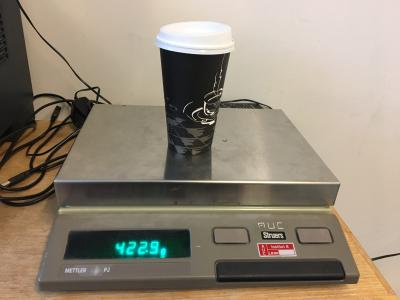
\includegraphics[width=0.45\textwidth, height=5cm]{Figures/Technical_figures/image3.jpg}
    \caption{A cup of tea weighing 422.9g}
    \label{fig:Tea}
\end{figure}
\columnbreak
\begin{figure}[H]
    \centering
    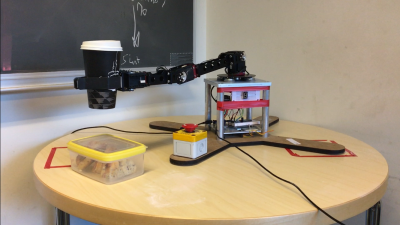
\includegraphics[width=0.45\textwidth,height=5cm]{Figures/Technical_figures/image4.png}
    \caption{The manipulator holds the cup in a streched out posistion.}
    \label{fig:stretch}
\end{figure}
\end{multicols}

\subsection*{Layout}
The sEMG electrodes will be attached as in section \ref{test:Connectiontest} and used to control the manipulator.
The manipulator will be moved to a stretched position as seen in figure \ref{fig:stretch} and the the weighted cup will be placed in the end effector as seen in figure \ref{fig:Tea}. 
\subsection*{Success criteria}
To succeed the manipulator needs to lift an object with a mass of $500g$
\subsection*{Iterations}
\begin{enumerate}
    \item The first test was done with a 523g bottle, this was to measure if it could lift over $500g$, but it failed.
    \item Test nr.2 was done with a cup of $500g$, which failed. 
    \item The previous tests failed, so it was decided to use a cup with the equivalent mass of a standard cup of tea ($422.9g$)  and test the PWM signal instead. The PWM signal is set to 200 at the start of this test. First the robot was not able to lift the cup, therefore, the PWM signal is set to 250.
    \item This was still not enough, so the PWM is set to 300. 
    \item Same as in iteration 2, and the PWM is set to 350.
    \item A PWM of 350 is almost enough.
    \item PWM was set to 360, the robot could now move the elbow joint to lift the cup.
\end{enumerate}
\subsection*{Result}
The manipulator succeeded in raising the cup of tea, which measured 422.5g. The requirement of lifting $500g$ is not met, however, the result is satisfactory. Furthermore the PWM threshold was decided and calibrated.\\
This test complies with requirement R\ref{req:extension}
\newpage
\testing{IMU Test R\ref{req:imu}}
\subsection*{Layout}
This test is done with the same layout as in Section \ref{test:Connectiontest}. The goal of this test is to fine-tune the motor select function in the system. 
\subsection*{Success criteria}
 The robot must be able to reliably switch the active joint based on the data from the IMU. This means that the user must be able to select the desired joint in both directions 10 times in a row.
\subsection*{Iterations}
\begin{enumerate}
    \item First the accelerometer thresholds has to be set for the individual test person. Incorrect thresholds makes it difficult to reach the desired motor. 
    \item The motor-ID jumps from 4 to 1 in one acceleration, which makes it problematic shifting the motor correctly. By adding a delay of 30 milliseconds this problem can be solved.
\end{enumerate}
\subsection*{Result}
It is clearly important to get the thresholds right during the setup. With the use of multiple test persons we see that some can reach accelerometer values of 850 and others only 750. With the use of a graphical representation of the accelerometer-data one can find the thresholds by letting the test person do a movement. This allows to set a specific thresholds for each test person.
\newpage

\testing{Safety R\ref{req:electrocution}}
\subsection*{Layout}
 The measuring box is turn on will each electrode is plug in the measurement box. The user in this concept, will not be in direct contact with the robotic manipulator, so only a test of the safety will be done on the measuring box.
 \begin{figure}[H]
     \centering
     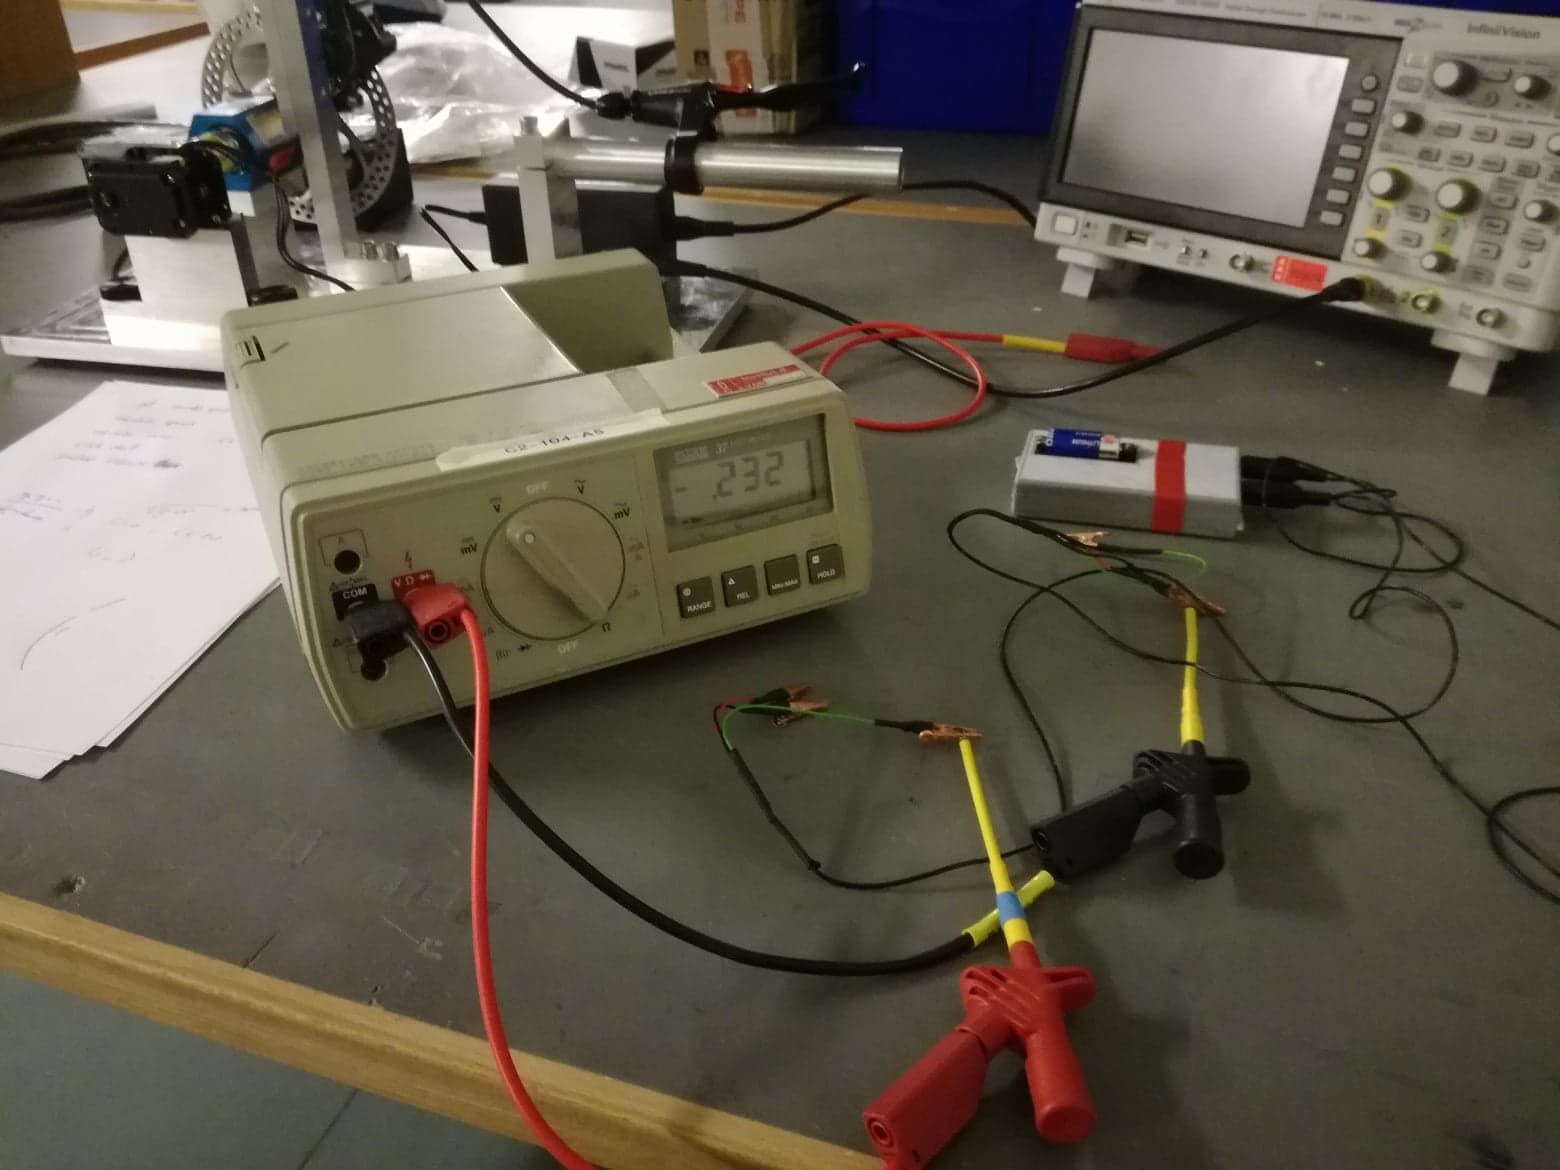
\includegraphics[width=0.45\textwidth, height=5cm]{Figures/Technical_figures/safetysetup.jpg}
     \caption{Setup of electrode measurement}
     \label{fig:my_label}
 \end{figure}
\subsection*{Success criteria}
 The Success criteria is that the will no to very low voltage measured across the electrodes which will ensure that there is no risk of be electrocuted. 

\subsection*{Result}
  Turning on the measuring box, and measuring the voltage level between the electrodes the group found a leak voltage of 0.23 volt, this is found not to be harmful and the measuring box is deemed safe for the user.   
 
\newpage

\testing{Latency R\ref{test:Latency}}
\begin{figure}[H]
    \centering
    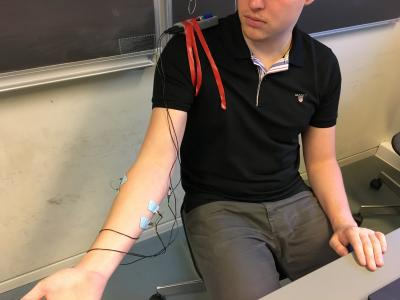
\includegraphics[width=10cm,height=5cm]{Figures/Technical_figures/image0.jpg}
    \caption{Electrodes and measuring box is mounted on the test person}
    \label{fig:connectiontest}
\end{figure}

\subsection*{Layout}
This test is done with the same layout as in Section \ref{test:Connectiontest}.
In order to calculate the system latency a video is recorded. The frame where the test persons movement start to the frame where the robot moves is found and the latency given as the time between the two frames. The latency must correspond to requirement: \ref{test:Latency}.

\subsection*{Success criteria}
 The robot must then be able to receive and act upon the signals from the measuring box. By switching the active joint on the robot using the IMU and turning in both directions using the EMG signal, and the robot must then be able to use that signal reliably and within 1 second.
\subsection*{Iterations}
\begin{enumerate}
    \item The connection was successful in the first iteration.
    \item Test 2 included a video of the test person, which is used to calculate the time it takes for a contraction to be uploaded to the manipulator.
\end{enumerate}
\subsection*{Result}
 It was clear that data was transferred since it was possible to move in the directions of choice and change the joint to move about this was recorded. 
  It was calculated trough the recording, that was analysed through a software program called \textit{"Tracker"}, the system had a latency of around 0.26 sec which was compliant with the requirement R\ref{test:Latency}. This was calculated by look at the amount of frames it took from the test person have activated a muscle to the manipulator moves. This happen within 8 frames the camera recording was at 30 frames per second.
\newpage

\testing{Forces of the robot R\ref{req:force}}

\begin{multicols}{2}
\begin{figure}[H]
    \centering
    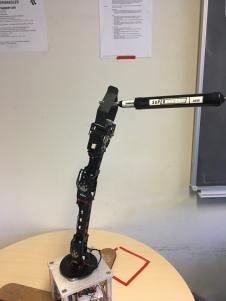
\includegraphics[width=0.45\textwidth, height=5cm]{Figures/Technical_figures/image5.jpg}
    \caption{The manipulator is pulled with a newton-meter to calculate the force in N}
    \label{fig:Nm}
\end{figure}
\columnbreak
\begin{figure}[H]
    \centering
    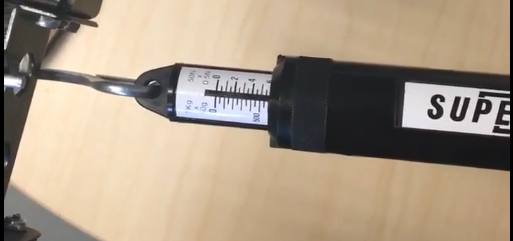
\includegraphics[width=0.45\textwidth,height=5cm]{Figures/Technical_figures/Capture.png}
    \caption{The manipulator pulls while the newton-meter is locked in a position.}
    \label{fig:pull}
\end{figure}
\end{multicols}
\subsection*{Layout}
The manipulator is preset to angles and PWM, which is 2000 for all the angles and 360 for the PWM. A newton-meter was used to measure all the forces on the joints, as seen in figure \ref{fig:Nm}.\\
In order to ensure the safety of the user, a second test is included in this section. The manipulator have to pull with the set PWM signal, by doing that it can be measured how much the manipulator will continue to pressure if a person is hit.
\subsection*{Success criteria}
We want the forces on all of the joints to be below 194.50N
\subsection*{Iterations}
\begin{enumerate}
    \item The first test decided how much force it was required to separate the fingers, which was 20N.
    \item The second test decided how much force it would take to rotate around the shoulder joint.
    The result was 14N
    \item The third test decided how much force it would take to rotate around the shoulder elbow joint. The result was 21N
    \item The fourth test decided how much force it would take to rotate around the shoulder base joint. The result was 14N
    \item The fifth test decided how much force the manipulator pressures with when it has hit a person. The result was 6N
    \end{enumerate}
\subsection*{Result}
Each separate joint is below the required N, which complies with requirement R\ref{req:force}.\\
\newpage

\testing{Final Test}

\begin{figure}[H]
    \centering
    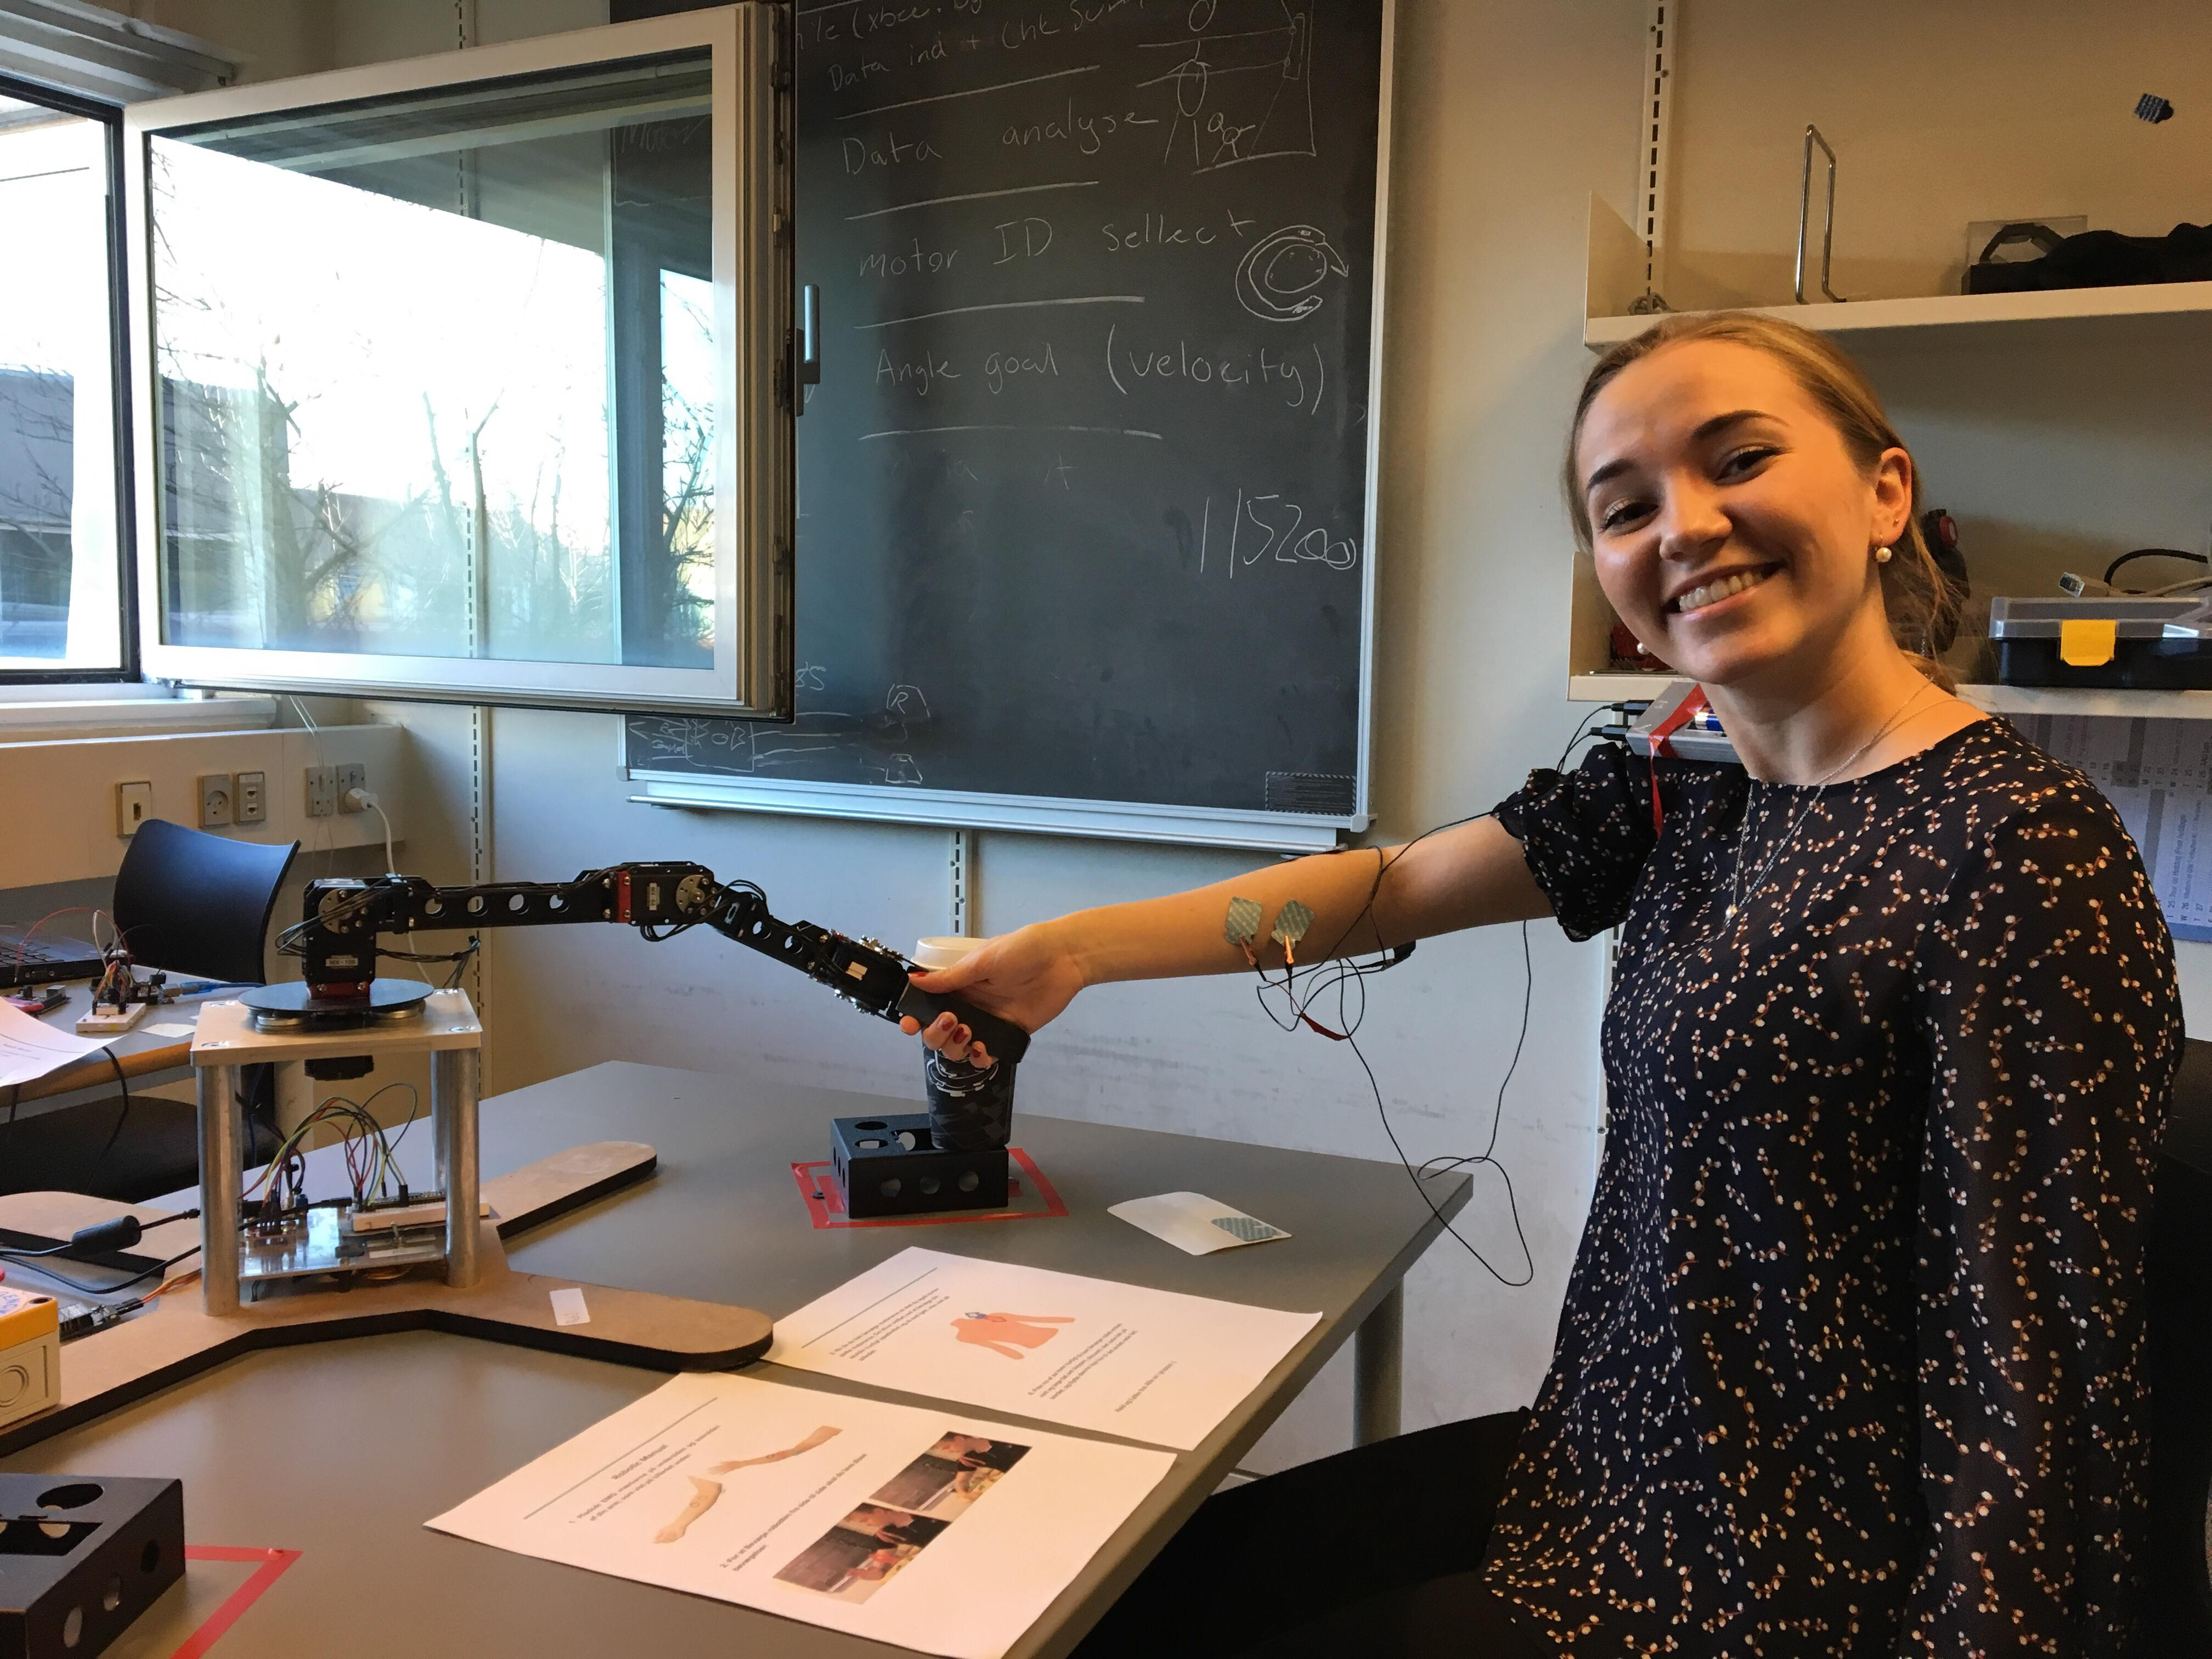
\includegraphics[width=8cm,height=5cm]{Figures/Technical_figures/anna.jpg}
    \caption{Anna Julie Qvist testing the robot}
    \label{fig:Anna}
\end{figure}

\subsection*{Layout}
This test is done with the same layout as in Section \ref{test:Connectiontest}. This time the manipulator is controlled by several people from outside the group to test if it is intuitive to use. 10 minutes is used to teach the system to the test person and for adjusting thresholds.
\subsection*{Success criteria}
 The test person have to use the manipulator to move a simulated standard cup of tea like in test \ref{sec:Lift}, in under 3 minutes. An exercise round is given to the test person so the person can get used to the contractions and accelerations. In the second test they have to do their best to move the cup under 3 minutes.
\subsection*{Iterations}
This test was done with multiple test persons. Four users that have never used the system and the four project group members. The table below show the result of the test for every test person, the experience level and the average time for that group. 
\begin{table}[H]
    \centering  
\begin{tabular}{ |P{2cm}||P{2cm}||P{3cm}||P{2cm}||P{3cm}|  }
 \hline
 \multicolumn{5}{|c|}{\textbf{Time spent on moving a cup}} \\
 \hline
 Person ID &Gender& Experience lvl & Time & Average time\\
 \hline
 \hline
 1 & Female & First time user & $3:56$ &   \\ \cline{1-4}
 2 & Male & First time user & $1:13$ &  2:28.25\\ \cline{1-4}
 3 & Female & First time user & $3:40$ &  \\ \cline{1-4}
 4 & Male & First time user & $1:04$ &  \\
 \hline\hline
 5 & Male & Expert & $0:40$ &   \\ \cline{1-4}
 6 & Male & Expert & $0:46$ &  0:48.5\\ \cline{1-4}
 7 & Male & Expert & $0:52$ &  \\ \cline{1-4}
 8 & Male & Expert & $0:56$ &  \\ \hline
\end{tabular}
\caption{Table of conditions and time used on moving a cup}
    \label{tab:UReq}
\end{table}
    %\item Anna Julie Qvist managed to use the manipulator and move the cup of tea in 3 minutes and 56 seconds. There was some minor disruptances with the EMG electrodes, otherwise the test person could have done it faster.
    %\item Peter-Ole Færgemand Managed to use the manipulator and move the cup of tea in 1 minutes and 13 seconds.
%\end{enumerate}
\subsection*{Result}
The average time spent by first time users is 2:28.25. This is well below the requirement of 3 minutes. Further more, it is clear that practice can improve that time significantly, since every group member was well below the average time of the first time user.The test persons didn't feel any inconveniences using the system and was easily able to use the manipulator. 



\section{Test Discussion} \label{sec:discuss}

Discussions of the test section leads to a better insight on what went wrong and what could have been done better.

\subsection*{Discussion of: Test 1 - EMG Thresholds}
Using EMG to control the rotations of the servos was a challenge. A lot of code was implemented but after a couple of months, the code was cracked. The test included the contractions of two muscles on the lower arm, it is acknowledged that the user is supposed to have a shoulder disarticulation, but since this is a proof of concept test arguably the electrodes could have been placed on two fresh muscles, e.g the chin muscles.\\
The user should then keep contracting the muscles in 3 minutes, although 3 minutes is not enough to conclude that the end user won't get tired after 10 hours with these contractions, it is enough to conclude that e.g a cup can be placed to drink from in that interval.\\
The user used some time to get the rotations of the of the servos right, but when the Thresholds were sat correctly and some practice of the contractions had been undergone the EMG worked intuitively like expected.\\
The thresholds were a different story, a lot of struggle and time went towards finding the right muscles to place the electrodes so that the contraction didn't have to take all the users strength before the CrustCrawler would move. After some time a GUI was found and utilised to get a better read on the EMG signal. Having a visual helped and the group was able to find the thresholds in a more efficient manner. Although the problem consists of finding the right place on the body for the electrodes and the threshold from person to person is different.
\paragraph{Conclusion:} Going through all these problems has made the CrustCrawler more intuitive, however the setup of the system and finding the persons EMG Thresholds can take some time. A solution to this can be only to have 1 user for 1 system.  

\subsection*{Discussion of: Test 2 - Lift Test}
The CrustCrawler had to undergo a trial of lifting a minimum of 500g; the number 500 is taken from an iso-standard of how much a general cup of tea weighs (420g), so the group decided to add a little extra weight so that different sizes of cups could be used.\\
The tests were unsuccessful with the extra added weight so it was decided to test the iso-standard as seen in the test. What could have been done? Well, a number of things could be done, such as: Not only testing on the joint which has to apply the most torque, and not testing it in a fully stretched position. Furthermore, the PWM could be altered to add more velocity on the pull it has to make to lift an object, but this could result on an uncontrollable movement in the upward direction and result in a spill of the hot cup of tea.\\
Although the group decided to leave it and accept the lift of the standard weight of a cup of tea.
\paragraph{Conclusion:} Alterations could have been made in the testing phase such as lifting the cup with other joints and require another position than "stretched out", lastly getting the correct PWM for the lift. However, it was decided to be acceptable to lift an iso-standard weighing cup of tea. However, counter-benefits was acknowledged by altering these things.

\subsection*{Discussion of: Test 3 - IMU Test}
The IMU in the "Measuring Box" was used to define the "Motor Select", stated in the sections above it moves in the Z-direction. Many considerations on how this went wrong have been done because the group witnessed and experienced a lot of failures in the thresholds and the placement of the IMU.\\
Besides that it is kind of annoying to keep accelerating one's shoulder in an upward direction it has been deemed hard to consider different peoples acceleration of the shoulder, some do it way too slow and then trigger a downward acceleration, which results in an opposite motor switch. After testing the acceleration on different persons, it has come to our knowledge that it takes a lot of time to redefine different thresholds because it is also hard for the user to keep accelerating with the same speed all the time. However, a fix was introduced in late November that saved the "motorSelect" function. By adding millis(), as a function to delay the function, the user could then only switch motors in every 3 seconds. The problem of levelling the threshold to fit different persons still consists.
\paragraph{Conclusion:} By altering the function, which switches the motor, with a time function before it can be run again fixed the problem, which almost consisted throughout the semester. The thresholds of the acceleration continues to be a struggle when introducing it to new users. However, adjusting it to one user can fix this problem.

\subsection*{Discussion of: Test 4 - Safety}
Safety for the user is large aspect due to a wide varieties of issues as force the manipulator applies or how it is fitted to the user. In this test, the project group focus mainly on the consideration of electricity, and making sure that the user never are exposed to any form of voltage the hurt them or in worst case scenario kill them through electrocution.\\
Due to the fact that of this only a concept the 12 volt power supply for the CrustCrawler, was not considered switched for battery source, if a battery would be implemented, it would have to be reliable and safe, a battery packs a lot of stored energy and can cause major damaged and fire if not handled correctly.
\paragraph{Conclusion:}
It was concluded that voltage level that user could experience, was at a maximum of 3 volt that comes from the battery that supplies the measuring box. all tho it was never measured on the electrodes.

\subsection*{Discussion of: Test 5 - Latency}
The connection test is crucial to test if the robot understands the signals sent to it.\\
Matlab was used in the first 2 months, where the connection from the Xbee was sent through the computer first and then into the CrustCrawler. Using several key components such as the computer, the Xbee and the CrustCrawler, made things complicated. After 100+ tries to make these key components work together, and creation of GUI's, it became clear to skip the MATLAB program and work with Arduino instead, which the group have worked with before.\\
Why did the MATLAB fail? One consideration that has been thought about is the fact that the RS-232 doesn't consider queues sent by MATLAB. By ignoring these queues it will send 8-bits, then ignore the rest and send 8-bit more, while MATLAB "spams" the wire with data. This means that the correct data will not always be implemented in the CrustCrawler.
\paragraph{Conclusion:} It became clear that the conversion from MATLAB to Arduino should have been done earlier.

\subsection*{Discussion of: Test 6 - Force of the robot}
Using a newton-meter to force the different joints to rotate is a really unreliable method of testing the force. However, the need to be precise in this particular test is not the priority. The priority is to estimate of much force it would take to bend the joints when the robot is pushing, which all were below the required force as stated in the test.\\
The fact that the CrustCrawler still could be a danger has been taken into consideration. Although the force isn't dangerous to be hit with, this low force could still be a danger if the CrustCrawler had a sharp object in its end-effector. As a result of this, a quick solution could be to loosen the grip of the end-effector so the object would slide out of the hand when pressed against something harder than expected. However, this is only a test of the force the CrustCrawler can bend away with when pressing into a person.
\paragraph{Conclusion:} Even though the CrustCrawler is not a danger when considering bending off when pressure is applied from the servos, the CrustCrawler should still be considered dangerous if given a sharp object to hold in the end-effector.

\subsection*{Discussion of: Test 7 - Final Test}
As read in the discussions above the problem consists of setting thresholds when different people are using the system. Excluding the setup, the users were impressed by the invention, and the group got a lot of useful feedback, like, LED's on the motors to get a better view on which motors were switched to.\\
A manual was presented to the users to see if they could operate the manipulator all by themselves, excluding the threshold setup. Doing that one of the test persons could figure it out but it were decided by the group that it was not intuitive enough and that this was a job for the manufacturer.\\
Lastly, the test was done on both layman, and project members themselves. An average  of the layman was done to analyse if the control system was intuitive. 
\paragraph{Conclusion:} By testing the system on several users, the group can get a better understanding of how intuitive the system is and how much time is spent on doing a simple task. By having most test persons under 3 minutes, the group has deemed the system useful and intuitive.